\section{Repeated Games}
Till now, the games or situations that were being considered were on a one-time basis, ie. the players faced each other once and moved on. But what happens in real life is there is constant day-to day interactions between the players and that adds up to more than just a single matchup. Hence, we need to repeat the situations and understand the changes that occur in the actions available as well as undertaken by them.

\subsection{Infinitely Repeated Games: Utitlity}
In this, we have a normal form game, and the players play that game over and over again. That means that each player gets a sequence of payoffs that is infinite, and hence cannot use the utility theory to understand it. We can't write it in extensive form as there will be no leaf node for the infinitely deep payoff. Also, we cannot sum up the sequence of payoffs and define utility to be the sum,  because it would be unbounded, and we want a finite one. Instead, we can use the following definition:-\\
\newline
Given an infinite sequence of payoffs $r_1, r_2, \dots$ for player $i$, the \textbf{average reward} for $i$ is $$\lim_{x\to \infty} \sum_{j=1}^{k} \frac{r_j}{k}$$
But technically, this method isn't quite well defined. For example, a player receives a negative payoff early on for a long time,  maybe $100,000$ iterations and positive for the rest, which would result in a positive average reward overall, but hides the fact that the negative payoff early on might be a deal breaker. Hence, we define the term \textbf{discounted reward} as follows:-\\
\newline
Given an infinite sequence of payoffs $r_1, r_2, \dots$ for player $i$ and the discount factor $\beta$ with $0 < \beta < 1$, $i$'s \textbf{future discounted reward} is $$\sum_{j=1}^\infty \beta^j r_j$$
Here the discount factor talks about the value of payoffs for different times.\\
\newline
Two equivalent interpretations of discount factor:
\begin{enumerate}
\item The agent cares more about his well-being in the near term than in the long term
\item The agent cares about the future as much as the present , but with probability $1-\beta$ the game will end in any given round
\end{enumerate}

\subsection{Stochastic Games}
\textbf{Formal Definition:}\\
\newline
A \textbf{stochastic game} is a tuple $(Q, N, A, P, R)$ where-
 
\begin{itemize}
\item $Q$ is a finite set of states
\item $N$ is a finite set of $n$ players
\item $A = A_1 \times \dots \times A_n$ where $A_i$ is a finite set of actions available to player $i$
\item $P: Q \times A \times Q\to [0,1]$ is the transition probability function; $P(q, a, \hat q)$ is the probability of transitioning from state $q$ to $\hat q$ after joint action $a$
\item $R = r_1, \dots, r_n$ where $r_i:  Q \times A \to \mathbb{R}$ is a real valued payoff function for player $i$
\end{itemize}
A stochastic game is a generalization of repeated games where-
\begin{itemize}
\item agents repeatedly play games from a set of normal form games
\item the game played at any iteration depends on the previous game played and on the actions taken by all agents in that game
\end{itemize}
 \begin{center}
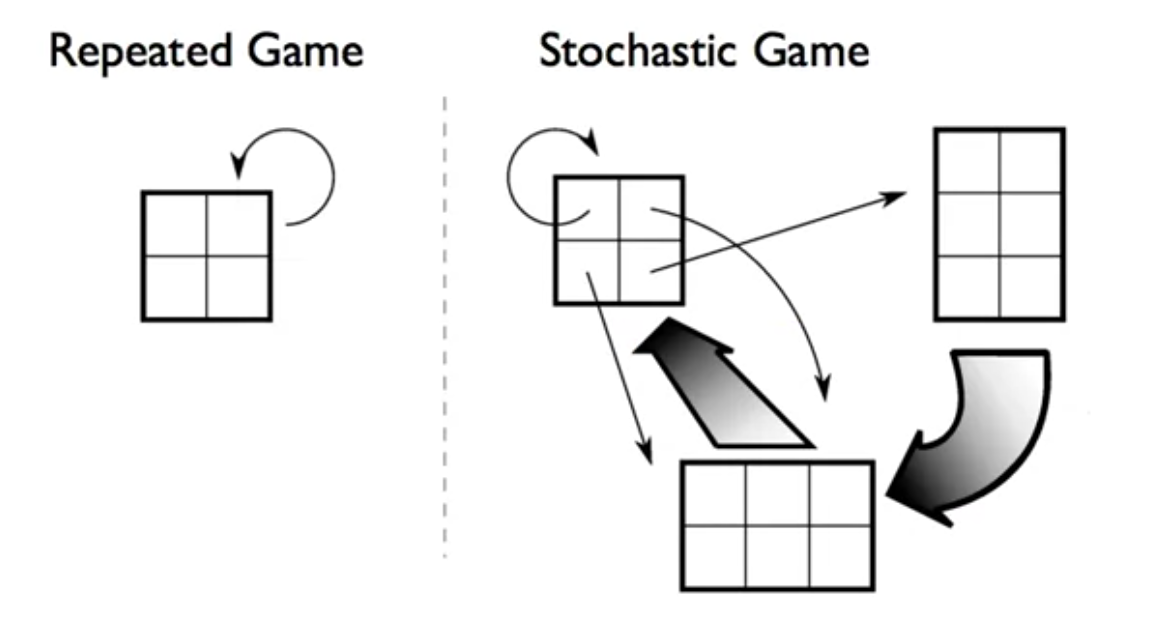
\includegraphics[scale=0.5]{stochastic}\\
An informal visualisation of the  difference between repeated and stochastic games
\end{center}
\subsection{Infinitely Repeated Games: Equilibria}
In an infinitely repeated game your strategy is going to be a choice of action at every decision point that you would have, which means an action that you would take every stage game. And when you take those actions, you actually get to reason about everything that you've seen before in the game ,that is, you can remember all of your own previous actions and you can also remember all of the actions in previous stage games by other players.\\
\newline
So, your pure strategy space is mapping from every history to an action choice that you would make. Clearly, this is an infinite number of actions. So, unlike the previous games we've looked at, extensive form games and normal form games, you're not even going to have a finite set of pure strategies in an infinitely-repeated game.

Some famous pure strategies in such case for Prisoners' Dilemma can be:-
\begin{itemize}
\item \textbf{Tit-for-tat}: Start out cooperating. If the opponent defected, defect in the next round. Then go back to cooperation
\item \textbf{Trigger}: Start out cooperating. If the opponent ever defects, then defect forever
\end{itemize}

\textbf{Some Notations:}\\

Consider any $n$-player game $G = (N, A, u)$ and any payoff vector $r = r_1, r_2, \dots , r_n$\newline
Let $v_i = min_{s_{-i}\in S_{-i}} max_{s_i \in S_i} u_i(s_{-i}, s_i)$\\
$i$'s minimax value: the amount of utility $i$. can get when $-i $ play a minimax strategy against him\\

\textbf{Defintion}:
\begin{itemize}
\item A payoff profile $r$ is \textit{enforceable} if $r_i \geq v_i$
\item A payoff profile $r$ is \textit{feasible} if there exists rational, non-negative values $\alpha_a$ such that for all $i$, we can express $r_i$ as $\sum_{a\in A} \alpha_a u_i(a) $ with $\sum_{a\in A} \alpha_a = 1$
\end{itemize}

\subsubsection{Folk Theorem}

Consider any $n$-player game $G$ and any payoff vector $(r_1, r_2, \dots, r_n)$.
\begin{itemize}
\item If $r$ is the payoff in any Nash equilbrium of the infinitely repeated $G$ with average rewards, then for each player $i$, $r_i$ is enforceable
\item If $r$ is both feasible and enforceable, then $r$ is the payoff in some Nash Equilibrium of the infinitely repeated $G$ with average rewards
\end{itemize}

\subsection{Discounted Repeated Games}
\textbf{Notations:}
\begin{itemize}
\item \textbf{Stage game}: $(N, A, u)$
\item \textbf{Discount Factors}: $\beta_1, \dots, \beta_n, \beta_i \in [0,1]$
\item \textbf{Assume a common discount factor} $\beta_i = \beta$ for all $i$
\item \textbf{Payoff from a play of actions} $a^1, \dots , a^t, \dots:$ $$\sum_t \beta_i^t u_i(a^t)$$
\end{itemize}
\textbf{Histories:}
\begin{itemize}
\item \textbf{Histories of length }$t$: $H^t = \{h_t : h^t = (a_1, \dots, a_t) \in A^t\}$
\item \textbf{All finite histories}: $H = \cup_t H^t$
\item \textbf{A strategy:} $s_i: H \to \Delta(A_i)$ 
\end{itemize}

\subsubsection{Repeated Prisoners' Dilemma}
\begin{itemize}
\item Cooperate as long as everyone has in the past
\item Both players defect forever after if everyone ever deviates: \textit{Grim Trigger}
\end{itemize}
Consider the following matrix:
\begin{center}\begin{tabular}{|c|c|c|} \hline
1/2 & $C$ & $D$ \\ \hline
$C$ & 3,3 & 0,5 \\ \hline
$D$ & 5,0 & 1,1 \\ \hline 
\end{tabular}\end{center}
\begin{itemize}
\item Cooperate from start: $3 + \beta \times 3 + \beta^2 \times 3 + \beta^3 \times 3 \dots = \frac{3}{1-\beta}$
\item Defect from start: $5 + \beta \times 1 + \beta^2 \times 1 + \beta^3 \times 1 \dots = 5 + \beta \times \frac{1}{1-\beta}$
\item Difference : $\beta \times \frac{2}{1-\beta} - 2$
\end{itemize}
The difference is non-negative if $\beta \geq \frac{1}{2}$. So, as long as people care about tomorrow, atleast half as much as today, they're going to be willing to cooperate in this.

But if we increase the incentive to defect from $5$ to $10$, the difference becomes $\beta \frac{2}{1-\beta} -  7$. Which means $\beta \geq \frac{7}{9}$ for the difference to be non-negative, which justifies the intuition that the agent has more urge to defect now than before. 
\subsubsection{Folk Theorem for Discounted Repeated Games}
Consider a finite normal form game $G = (N, A, u)$. Let $a = (a_1, \dots , a_n) $ be a Nash equilibrium of the stage game $G$.\\

If $a'= (a'_1, \dots, a'_n)$ is such that $u_i(a') > u_i(a)$ for all $i$, then there exists a discount factor $\beta < 1$, such that if $\beta_i \geq \beta$ for all $i$, then there exists a subgame perfect equilibrium of the infinite repetition of $G$ that has $a'$ played in every period on the equilibrium path